\documentclass[tikz, border=20pt, convert={density=300,outext=.png}]{standalone}
\usetikzlibrary{positioning, arrows.meta, fit, backgrounds, calc}

\begin{document}
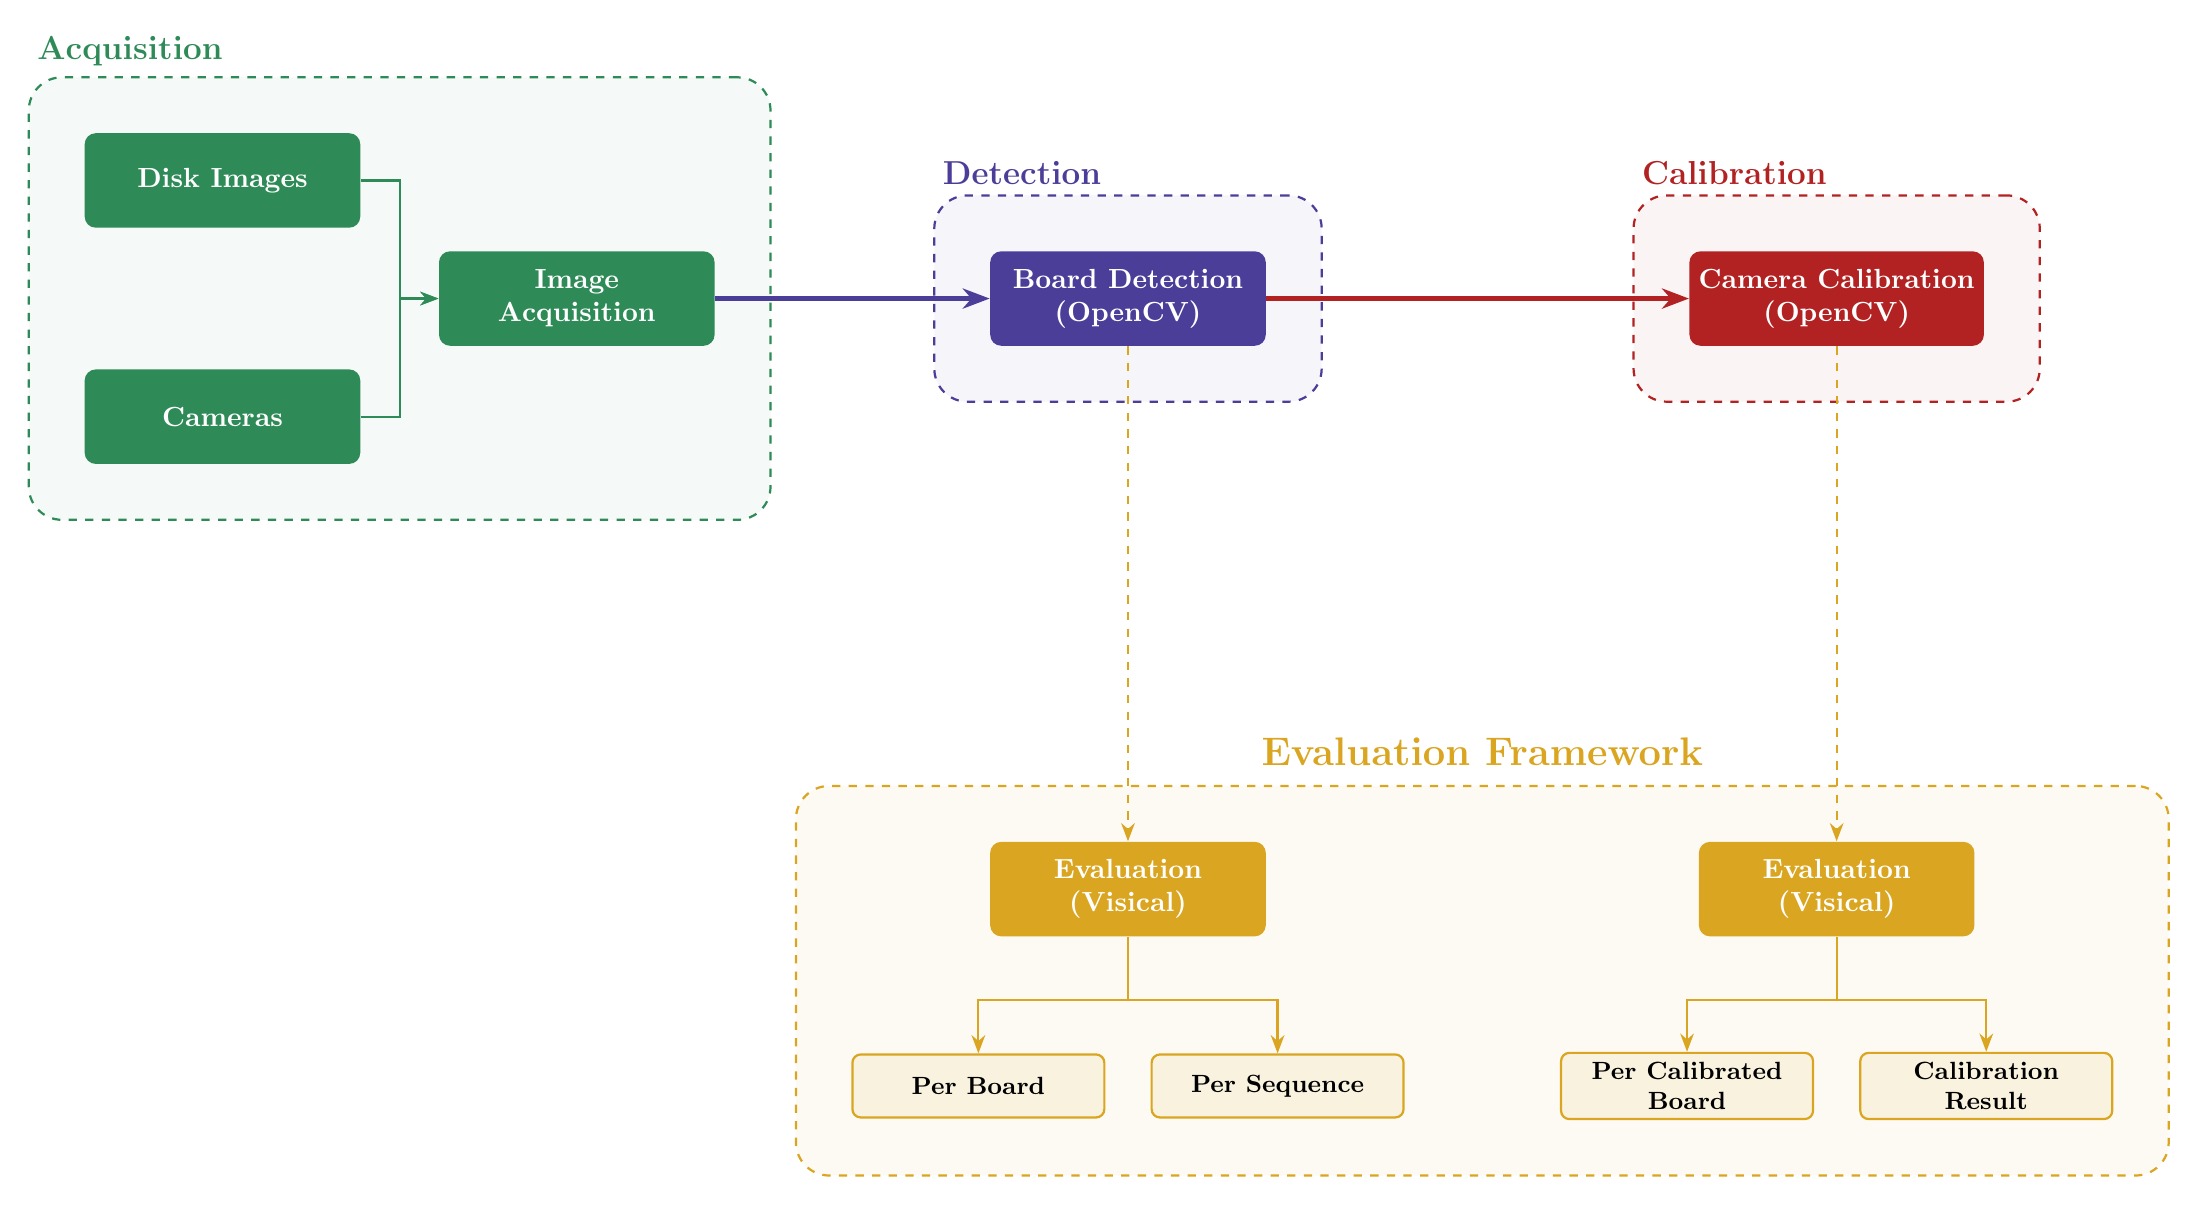
\begin{tikzpicture}[
    >=Stealth,
    font=\sffamily,
    mainnode/.style={rectangle, rounded corners=4pt, text=white, align=center, minimum width=3.5cm, minimum height=1.2cm, font=\bfseries},
    subnode/.style={rectangle, rounded corners=3pt, draw=#1, fill=#1!15, text=black, align=center, minimum width=3.2cm, minimum height=0.8cm, font=\small\bfseries, thick},
    layerbox/.style={rectangle, draw=#1, fill=#1!5, dashed, thick, rounded corners=12pt, inner xsep=20pt, inner ysep=20pt},
]

\definecolor{cAcq}{HTML}{2E8B57}  % Verde 
\definecolor{cDet}{HTML}{4b3e99}  % Blu/Viola
\definecolor{cCal}{HTML}{B22222}  % Rosso 
\definecolor{cEval}{HTML}{DAA520} % Giallo scuro/Oro 

\node[mainnode, fill=cAcq] (acq) at (0, 0) {Image\\Acquisition};
\node[mainnode, fill=cAcq] (disk) at (-4.5, 1.5) {Disk Images};
\node[mainnode, fill=cAcq] (cam)  at (-4.5, -1.5) {Cameras};

\node[mainnode, fill=cDet] (det) at (7, 0) {Board Detection\\(OpenCV)};
\node[mainnode, fill=cCal] (cal) at (16, 0) {Camera Calibration\\(OpenCV)};

\node[mainnode, fill=cEval] (eval_det) at (7, -7.5) {Evaluation\\(Visical)};
\node[subnode=cEval] (det_board) at (5.1, -10) {Per Board};
\node[subnode=cEval] (det_seq)   at (8.9, -10) {Per Sequence};

\node[mainnode, fill=cEval] (eval_cal) at (16, -7.5) {Evaluation\\(Visical)};
\node[subnode=cEval] (cal_board) at (14.1, -10) {Per Calibrated\\Board};
\node[subnode=cEval] (cal_res)   at (17.9, -10) {Calibration\\Result};

\node[font=\Large\bfseries, text=cEval] at (11.5, -5.75) {Evaluation Framework};

\draw[->, thick, cAcq] (disk.east) -| (-2.25, 0) -- (acq.west);
\draw[->, thick, cAcq] (cam.east)  -| (-2.25, 0) -- (acq.west);

\draw[->, line width=1.5pt, cDet] (acq.east) -- (det.west);
\draw[->, line width=1.5pt, cCal] (det.east) -- (cal.west);

\draw[->, dashed, thick, cEval] (det.south) -- (eval_det.north);
\draw[->, dashed, thick, cEval] (cal.south) -- (eval_cal.north);

\draw[->, thick, cEval] (eval_det.south) -- ++(0,-0.8) -| (det_board.north);
\draw[->, thick, cEval] (eval_det.south) -- ++(0,-0.8) -| (det_seq.north);

\draw[->, thick, cEval] (eval_cal.south) -- ++(0,-0.8) -| (cal_board.north);
\draw[->, thick, cEval] (eval_cal.south) -- ++(0,-0.8) -| (cal_res.north);

\begin{scope}[on background layer]
    \node[layerbox=cAcq, fit=(disk) (cam) (acq), label={[font=\large\bfseries, text=cAcq, anchor=south west]north west:Acquisition}] (bg_acq) {};
    \node[layerbox=cDet, fit=(det), label={[font=\large\bfseries, text=cDet, anchor=south west]north west:Detection}] (bg_det) {};
    \node[layerbox=cCal, fit=(cal), label={[font=\large\bfseries, text=cCal, anchor=south west]north west:Calibration}] (bg_cal) {};
    \node[layerbox=cEval, fit=(eval_det) (det_board) (det_seq) (eval_cal) (cal_board) (cal_res)] (bg_eval) {};
\end{scope}

\end{tikzpicture}
\end{document}